\chapter{Laboratorium III}\label{ch:lab3}

\section{Wybrany sprzęt}\label{sec:lab3-hw}

Podobnie do~poprzedniego laboratorium, w~tym~przypadku również~jest~wykorzystany \emph{Grove Base Kit}.
Dzięki umieszczeniu tych~laboratoriów sąsiednio w~kolejności numerycznej oszczędzona~jest niewielka ilość czasu
na~zmiany połączeń fizycznych.

Głównym elementem laboratorium jest~czujnik ruchu \emph{mini PIR S16-L221D} kompatybilny ze~środowiskiem Grove.
Czujnik~ten umożliwia wykrywanie ruchu obiektów emitujących promieniowanie podczerwone.
Podłączony do~portu cyfrowego, jego użycie polega na~analizie zboczy sygnału wyjściowego.

W~laboratorium użyty został również przycisk z~diodą LED\@.
Dioda została wykorzystana do~sygnalizacji wykrycia ruchu przez czujnik, przycisk resetuje jej stan.
W~ten sposób program wynikowy pełni rolę prostego systemu alarmowego, powiadamiającego o~uprzednim wystąpieniu ruchu
w~obserwowanej strefie.

\section{Rozwiązanie}\label{sec:lab3-sol}

Rysunek~\ref{fig:alarmlab} to~fragment instrukcji przedstawiający zadanie wykrycia wciśnięcia przycisku wyłączającego
diodę.
Oczywiste rozwiązanie zawiera pewną niedogodność, która~ujawnia~się po~uruchomieniu pętli głównej z~dużym opóźnieniem
czasowym.
Interakcja z~czujnikiem ruchu, pomimo podobnego kodu, nie~ma tego~problemu dzięki wykorzystaniu mechanizmu flagi.

\begin{figure}[H]
  \centering
  \includegraphics[width=0.9\linewidth]{media/alarm_lab}
  \caption{Fragment instrukcji ``Alarm''}
  \label{fig:alarmlab}
\end{figure}

Rysunek~\ref{fig:alarm} przedstawia rozwiązanie zadania.
Czujnik ruchu został wywołany i~w~wyniku tej~akcji została uruchomiona dioda.
Z~powodu interaktywności zadania zdjęcie nie~jest idealnym sposobem przedstawienia działania.

\begin{figure}[H]
  \centering
  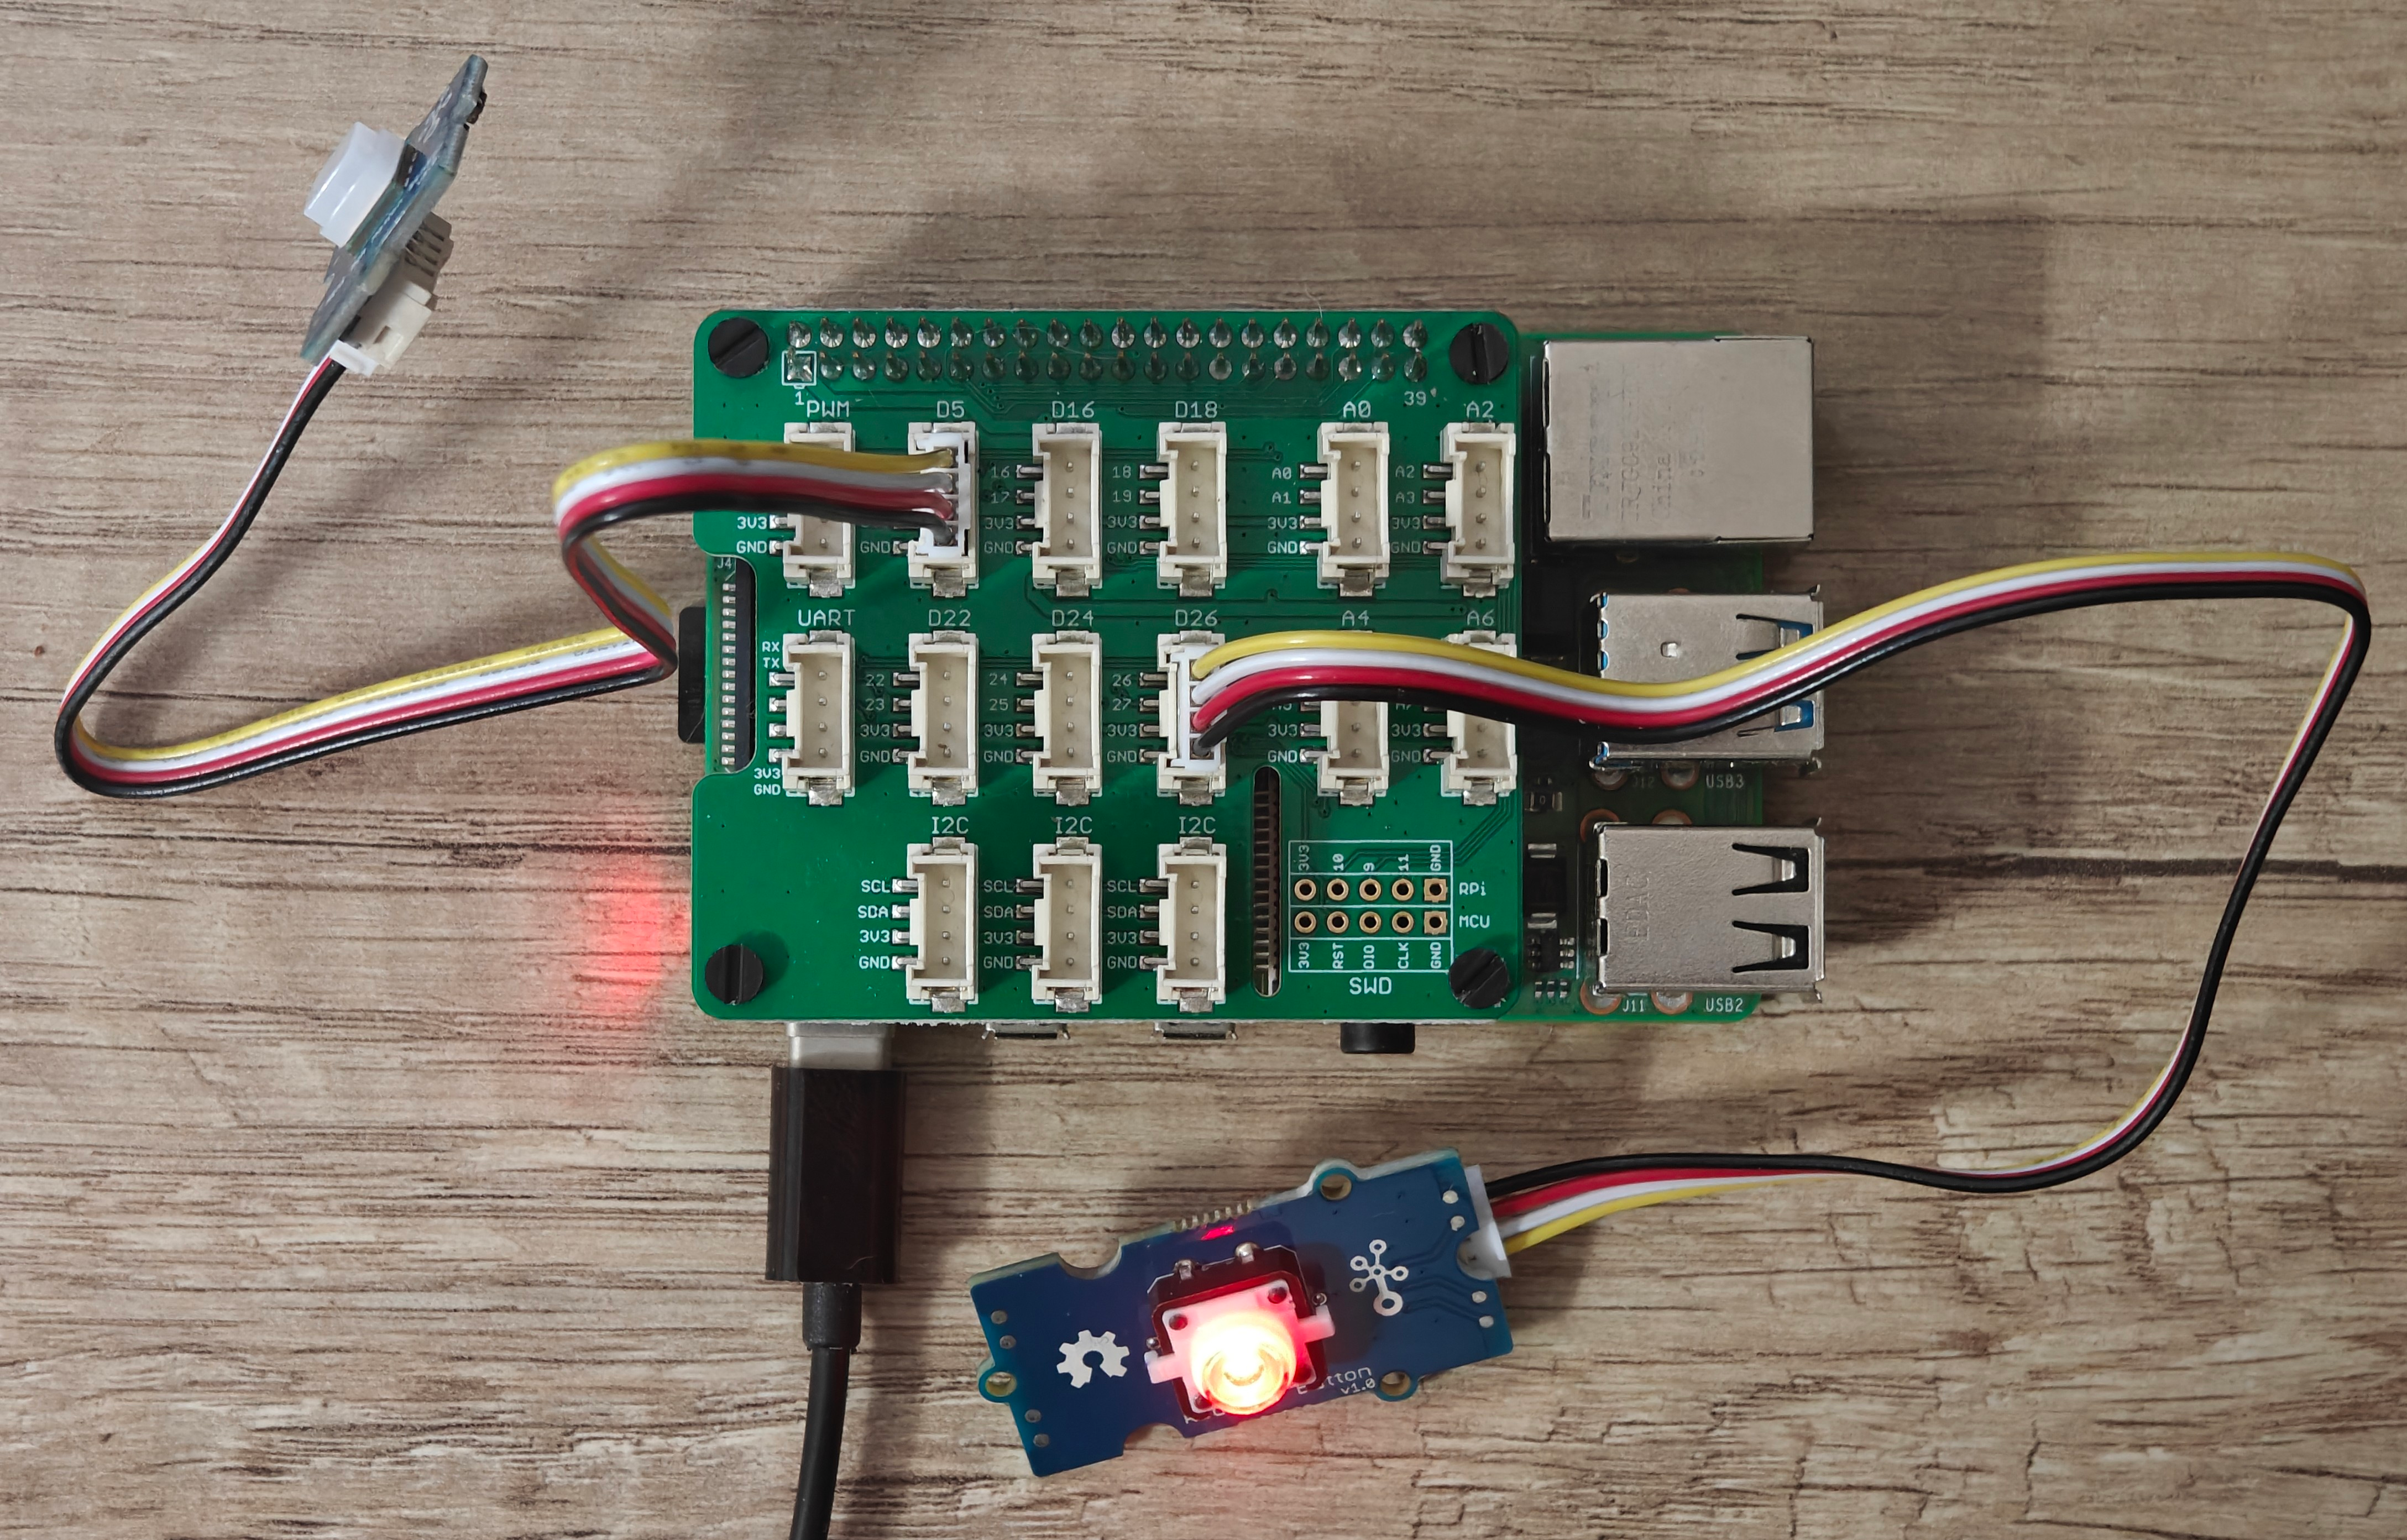
\includegraphics[width=0.6\linewidth]{media/alarm}
  \caption{Uruchomiony program trzeciego laboratorium}
  \label{fig:alarm}
\end{figure}
